%%%%%%%%%%%%%%%%%%%%%%%%%%%%%%%%%%%%%%%%%%%%%%%%%%%%%%%%
%%%%%%%%%%%%%%%%%%%%%%%%%%%%%%%%%%%%%%%%%%%%%%%%%%%%%%%%
%%%%%%%%%%%%%%%%%%%%%%%%%%%%%%%%%%%%%%%%%%%%%%%%%%%%%%%%
\chapter{Dimensionality Reduction}
\label{chap:dim_reduct}

%%%%%%%%%%%%%%%%%%%%%%%%%%%%%%%%%%%%%%%%%%%%%%%%%%%%%%%%
%%%%%%%%%%%%%%%%%%%%%%%%%%%%%%%%%%%%%%%%%%%%%%%%%%%%%%%%
\section{Feature Selection}
\label{dim_reduct:feature_selection}
% TODO
% TODO Can look at correlation or mutual information between variables
% TODO could also use a chi2 test for independence between input variables and the dependent variable, see which ones might be useful. See https://scikit-learn.org/stable/modules/generated/sklearn.feature_selection.chi2.html

%%%%%%%%%%%%%%%%%%%%%%%%%%%%%%%%%%%%%%%%%%%%%%%%%%%%%%%%
\subsection{Forward and Backward Feature Selection}
\label{dim_reduct:feature_selection:forward_backward}
% TODO

%%%%%%%%%%%%%%%%%%%%%%%%%%%%%%%%%%%%%%%%%%%%%%%%%%%%%%%%
%%%%%%%%%%%%%%%%%%%%%%%%%%%%%%%%%%%%%%%%%%%%%%%%%%%%%%%%
\section{Principle Component Analysis (PCA)}
\label{dim_reduct:PCA}
% https://youtu.be/dhK8nbtii6I

Principle component analysis (PCA) \cite{pca} is a popular linear method
of reducing a dataset to a limited set of more descriptive dimensions.
PCA works by preforming a change of basis from
the dataset's original vector space to a new orthonormal basis which
minimizes the average squared distance between the data points and the basis vectors,
or equivalently\footnote{See
\href{https://stats.stackexchange.com/questions/32174/pca-objective-function-what-is-the-connection-between-maximizing-variance-and-m/136072\#136072}{this post}
for one proof.} maximizes the variance of the data in the new vector space.
See \cref{fig:dim_reduct:PCA:illustration} for an illustration of PCA in action.

To begin, we construct a $n \times m$ matrix $\mb{X}$
from the $n$ features and $m$ data points in the original vector space
with basis $\left\{\vu{e}_{i}\right\}$.
If we project the $\vb{x}_{j}$ data point on to
some new unit vector $\vu{u}_{i}$,
$\vb{x}_{j} \to \vu{u}_{i}\transpose \vb{x}_{j} \vu{u}_{i}$,
the variance of the data along $\vu{u}_{i}$ will be

\begin{subequations}\label{eq:PCA:variance}
\begin{align}
\variance{\mb{X} \vu{u}_{i}}
&= \frac{1}{m}\sum_{j=1}^{m} \left(
\vu{u}_{i}\transpose \vb{x}_{j}
-
\vu{u}_{i}\transpose \expval{\vb{x}}
\right)^{2}
= \frac{1}{m}\sum_{j=1}^{m} \left( \vu{u}_{i}\transpose \left(\vb{x}_{j} - \expval{\vb{x}}\right)\right)^{2}, \label{eq:PCA:variance:a} \\
&= \frac{1}{m}\sum_{j=1}^{m}
\vu{u}_{i}\transpose
\left(\vb{x}_{j} - \expval{\vb{x}}\right)
\left(\vb{x}_{j} - \expval{\vb{x}}\right)\transpose
\vu{u}_{i}
= \vu{u}_{i}\transpose \mb{M} \vu{u}_{i}, \label{eq:PCA:variance:M}
\end{align}
\end{subequations}

\noindent where $\mb{M}$ is
the covariance matrix\footnote{$M_{ij} = \cov{\mb{X} \vu{e}_{i}}{\mb{X} \vu{e}_{j}} = M_{ji}$,
see \cref{stats:corr_covar:covar_matrix}.
When the data is centered and $\expval{\vb{x}} = \va{0}$,
$\mb{M} = \frac{1}{m} \mb{X} \mb{X}\transpose = \frac{1}{m} \mb{X}\transpose \mb{X}$.
Note that $\mb{X}\transpose \mb{X} \propto \mb{M}$
is commonly used in PCA derivations.} of $\mb{X}$
and $\expval{\vb{x}} = \sum_{i=1}^{n} \expval{\mb{X} \vu{e}_{i}} \vu{e}_{i}$.
We now wish to find a new orthonormal basis $\left\{\vu{u}_{i}\right\}$
which maximizes $\variance{\mb{X} \vu{u}_{i}}$,
subject to the constraint that $\abs{\vu{u}_{i}} = \vu{u}_{i}\transpose \vu{u}_{i} = 1$,
\ie the classic Lagrange multiplier problem of \cref{opt:lagrange_mult}.

Taking matrix derivatives

\begin{subequations}\label{eq:PCA:lagrange}
\begin{align}
0 &= \dv{\vu{u}_{i}} \left( \vu{u}_{i}\transpose \mb{M} \vu{u}_{i}
+ \lambda \left( 1 - \vu{u}_{i}\transpose \vu{u}_{i} \right) \right)
= 2 \mb{M} \vu{u}_{i} - 2 \lambda \vu{u}_{i}, \label{eq:PCA:lagrange:setup} \\
&\implies \mb{M}\vu{u}_{i} = \lambda \vu{u}_{i}, \label{eq:PCA:lagrange:eigen}
\end{align}
\end{subequations}

\noindent we discover that $\left\{\vu{u}_{i}\right\}$
is just the eigenbasis of $\mb{M}$ with eigenvalues $\lambda_{i}$.
If we left multiply \cref{eq:PCA:lagrange:eigen} by $\vu{u}_{i}\transpose$
we see that the eigenvalues $\lambda_{i}$ are actually the variances along the eigenvectors $\vu{u}_{i}$.
The eigenvector, $\vu{u}_{1}$, with the largest eigenvalue, $\lambda_{1}$, and thus largest variance
is known as the first principle component (PC1),
while the second largest variance $\lambda_{2}$ corresponds to $\vu{u}_{2}$,
the second principle component (PC2)\ldots

To actually perform the change of basis,
we construct $\mb{U}$ whose columns are the $\vu{u}_{i}$ eigenvectors
and then transform $\mb{X} \to\mb{U}\transpose \mb{X} = \widetilde{\mb{X}}$.
As we are typically performing PCA to reduce the dimensionality of the data,
we can select only the top $k$ principle components to keep, making
$\mb{U}\transpose_{k \times n} \mb{X}_{n \times m} = \widetilde{\mb{X}}_{k \times m}$.
Note that if there are few data points relative to the original dimensions, $m < n$,
the eigendecomposition of $\mb{M}_{n \times n}$ will still work, but some of the $\lambda_{i}$ may be $< 0$.
These eigenvalues should be disregarded, leaving $k \leq \min\left(m,n\right)$ possible principle components.

In practice, we should first center and rescale the data,
by subtracting the mean and dividing by the standard deviation along each dimension,
before preforming the eigendecomposition.
Intuitively, PCA is stretching and rotating the vector space to find the best principle components,
but the origin will remain fixed, $\vu{u}_{i}\transpose\,\va{0}\,\vu{u}_{i} = \va{0}$,
and the input dimensions are being mixed together $1 \mathbin{:} 1$ without regards for different units.
Some PCA software packages perform these preprocessing steps by default\footnote{For example,
{\sklearn}'s \texttt{PCA}
\href{https://scikit-learn.org/stable/modules/generated/sklearn.decomposition.PCA.html}{function}
only centers the data.
Scaling is handled by a separate transformation, as can be seen in
\href{https://scikit-learn.org/stable/auto\_examples/preprocessing/plot\_scaling\_importance.html}{this demo}.},
but it is not universal so check the appropriate documentation.

The computational algorithms used today to efficiently preform PCA are
frequently based on Singular Value Decomposition (SVD), see \cref{dim_reduct:SVD:PCA},
rather than a straightforward eigendecomposition of the covariance matrix.
Other related approaches include sparse PCA\footnote{Implemented
in \sklearn as the \texttt{SparsePCA}
\href{https://scikit-learn.org/stable/modules/generated/sklearn.decomposition.SparsePCA.html}{function}.
For more on this method, see the relevant \sklearn
\href{https://scikit-learn.org/stable/modules/decomposition.html\#sparsepca}{user guide section}.},
which incorporates a L1 regularization term to perform feature selection on the original $n$ dimensions,
removing those which are not needed to generate the leading $k$ principle components.

When modeling we should also take care to only run PCA on the training set,
to avoid utilizing any information from the test set.
Of course later while making predictions the same PCA transforms
will need to be applied before feeding data to the model.

\begin{figure}[H]
  \centering
  \savebox{\largestimage}{
    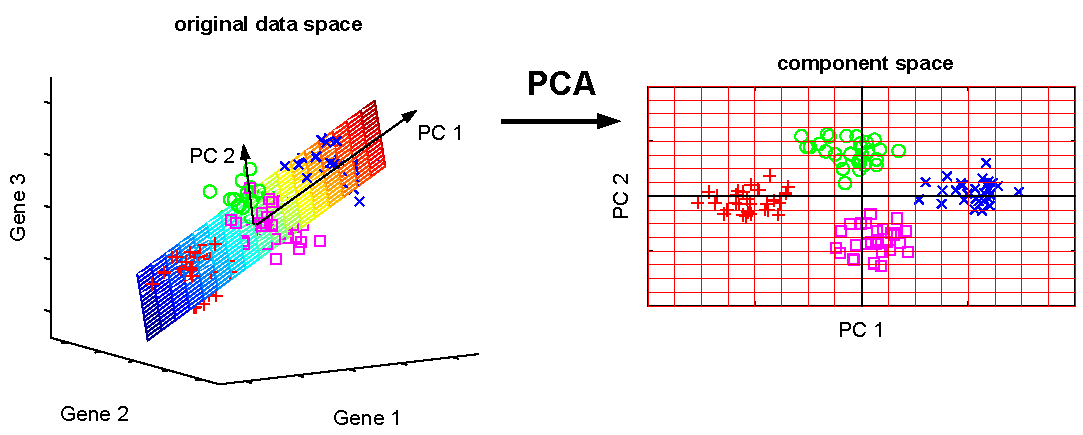
\includegraphics[width=0.47\textwidth]{figures/dim_reduct/fig_pca_illu3d}
  }% Store largest image in a box

  \begin{subfigure}[b]{0.48\textwidth}\centering
    \usebox{\largestimage}
    \vspace{0.01cm}
  \caption{PCA}
  \label{fig:dim_reduct:PCA:illustration}
  \end{subfigure}
  ~
  \begin{subfigure}[b]{\wd\largestimage}\centering
    \raisebox{\dimexpr.5\ht\largestimage-.5\height}{% Adjust vertical height of smaller image
      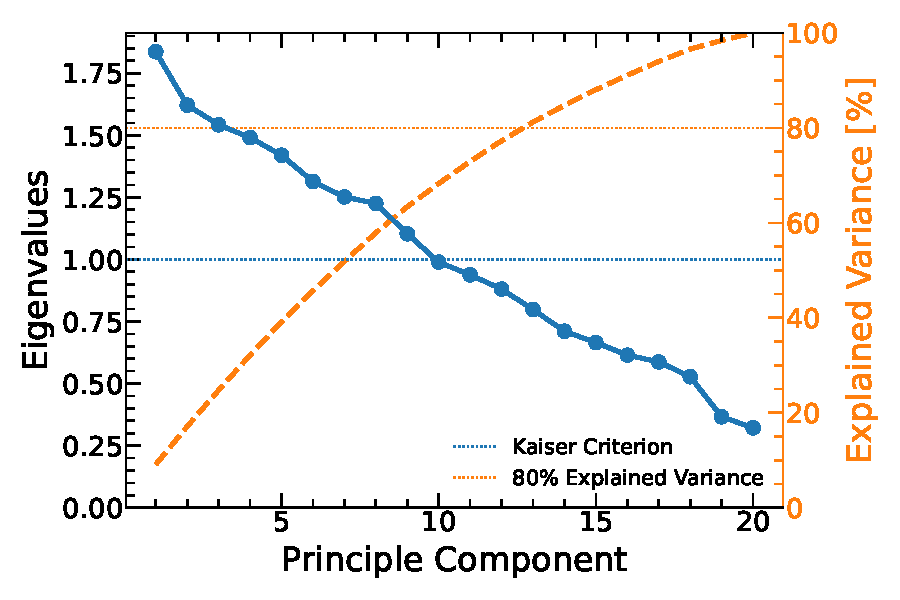
\includegraphics[width=\textwidth]{figures/dim_reduct/scree}}
  \caption{Scree Plot}
  \label{fig:dim_reduct:PCA:scree}
  \end{subfigure}
\caption{
On the left, an illustration of dimensionality reduction $m=3 \to k=2$ with PCA on genetics data \cite{Scholz2006}.
On the right, an example scree plot from a toy dataset.
Though there is no prominent elbow,
based on the Kaiser criterion (percent explainable variance)
we should consider reducing to $k=9$ ($k=13$) dimensions.
\label{fig:dim_reduct:PCA}
}
\end{figure}

%%%%%%%%%%%%%%%%%%%%%%%%%%%%%%%%%%%%%%%%%%%%%%%%%%%%%%%%
\subsection{Scree Plots}
\label{dim_reduct:PCA:scree}

When working with PCA we can use a
scree\footnote{Named after the similarly shaped geological feature, a rubble pile at the base of a cliff.} plot \cite{scree}
of the eigenvalues, such as \cref{fig:dim_reduct:PCA:scree},
to decide how many principle components to retain.
While this is always a somewhat subjective decision,
the Kaiser criterion \cite{kaiser_criterion} is one potential guideline,
keeping all principle components with $1 < \lambda_{i}$.
We can also look for an elbow in the plot,
or take the necessary principle components to reach
\si{80}{\percent} or $\si{90}{\percent} \leq \sum_{i=1}^{k} \lambda_{i} / \sum_{j=1}^{n} \lambda_{j}$ of the explainable variance.

%%%%%%%%%%%%%%%%%%%%%%%%%%%%%%%%%%%%%%%%%%%%%%%%%%%%%%%%
%%%%%%%%%%%%%%%%%%%%%%%%%%%%%%%%%%%%%%%%%%%%%%%%%%%%%%%%
\section{Singular Value Decomposition (SVD)}
\label{dim_reduct:SVD}
% https://youtu.be/HAJey9-Q8js
% https://www.youtube.com/watch?v=gXbThCXjZFM&list=PLMrJAkhIeNNSVjnsviglFoY2nXildDCcv

Singular value decomposition (SVD) is a linear method like PCA,
but it works directly on the data matrix $\mb{X}$,
rather than the covariance matrix $\mb{M}$.
We begin with the rectangular\footnote{Note that here we have constructed $\mb{X}$
with data points as row vectors, as in \cref{regression:linear},
while in \cref{dim_reduct:PCA} they were columns.
Though inconsistent, these definitions of $\mb{X} \leftrightarrow \mb{X}\transpose$
simplify the notation in each section.} $\mb{X}_{m \times n}$
of $m$ data points in the original $n$ dimensional vector space.
Let $\rank\left(\mb{X}\right) = r \leq \min\left(m,n\right)$.
We can then decompose $\mb{X}$ into $r$ linearly independent
rank 1 matrices $\vb{u} \vb{v}\transpose$ as

\begin{subequations}\label{eq:SVD}
\begin{align}
\mb{X} &= \sum_{i=1}^{r} \sigma_{i} \vb{u}_{i} \vb{v}_{i}\transpose, \label{eq:SVD:sum} \\
&= \begin{pmatrix}
  \vb{u}_{1} & \vb{u}_{2} & \ldots & \vb{u}_{r}
\end{pmatrix}
\begin{pmatrix}
  \sigma_{1} & 0          & \ldots & 0 \\
  0          & \sigma_{2} & \ldots & 0 \\
  \vdots     & \vdots     & \ddots & 0 \\
  0          & 0          & 0      & \sigma_{r}
\end{pmatrix}
\begin{pmatrix}
  \vb{v}_{1}\transpose \\
  \vb{v}_{2}\transpose \\
  \vdots \\
  \vb{v}_{r}\transpose
\end{pmatrix}\,, \label{eq:SVD:expanded} \\
&= \mb{U} \mb{\Sigma} \mb{V}\transpose, \label{eq:SVD:matrix_form}
\end{align}
\end{subequations}

\noindent where $\vb{u}_{m \times 1}$, $\vb{v}_{n \times 1}$,
$\mb{U}_{m \times r}$, $\mb{\Sigma}_{r \times r}$, and $\mb{V}_{n \times r}$.

As $\rank\left(\vb{u} \vb{v}\transpose\right) = 1$,
this implies that the $\vb{u}_{i}$ vectors are linearly independent, as are $\vb{v}_{i}$,
and thus\footnote{Here we are actually describing the ``compact'' form of SVD,
where $\mb{U}$ and $\mb{V}$ are not square, and thus are only semi-orthogonal
as $\mb{U} \mb{U}\transpose \neq \identity$, $\mb{V} \mb{V}\transpose \neq \identity$.
In regular SVD where $\mb{U}_{m \times m}$, $\mb{\Sigma}_{m \times n}$, and $\mb{V}_{n \times n}$,
$\mb{U}$ and $\mb{V}$ are orthogonal,
but $\mb{\Sigma}$ is only rectangular diagonal and $m-r$ of the singular values
are 0.} $\mb{U}\transpose \mb{U} = \mb{V}\transpose \mb{V} = \identity_{r \times r}$.
If they were not linearly independent,
we could not reconstruct $\mb{X}$ with $\rank\left(\mb{X}\right) = r$.
Rearranging \cref{eq:SVD:matrix_form} as

\begin{subequations}\label{eq:SVD:left_right}
\begin{align}
\mb{U}\transpose \mb{X} &= \mb{\Sigma} \mb{V}\transpose, \label{eq:SVD:left_right:left} \\
\mb{X} \mb{V} &= \mb{U} \mb{\Sigma}, \label{eq:SVD:left_right:right}
\end{align}
\end{subequations}

\noindent leads us to name the
$\vb{u}_{i}$ left-singular vectors,
$\vb{v}_{i}$ right-singular vectors,
and $\sigma_{i}$ singular values.
In this form, we see that SVD is a generalization of eigendecomposition to rectangular matrices.
We can also think of SVD as a form of generalized Fourier transform, expanding $\mb{X}$ into its components.

It can be shown\footnote{See the \href{https://en.wikipedia.org/wiki/Singular\_value\_decomposition\#Existence\_proofs}{SVD wikipedia page} for
existence proofs, and note we can reorder $\sigma_{i}$ as we like.} that
it is always possible construct a SVD of $\mb{X} \to \mb{U} \mb{\Sigma} \mb{V}\transpose$
with monotonically decreasing singular values $\sigma_{i}$, $\sigma_{i} > \sigma_{i+1}$.
We can thus approximate $\mb{X}$ by $\widetilde{\mb{X}}_{m \times n}$
having a lower $\rank\left(\widetilde{\mb{X}}\right) = k < r$
by setting $\widetilde{\sigma}_{i} = 0$ for $k < i$ in
$\widetilde{\mb{X}} = \mb{U} \widetilde{\mb{\Sigma}} \mb{V}\transpose$.
By the Eckart-Young theorem \cite{eckart1936}
this truncated SVD is the best rank $k$ approximation to $\mb{X}$,
minimizing the Frobenius norm\footnote{$\normF{\mb{X}}^{2} = \sum_{ij} \abs{x_{ij}}^{2} = \trace\left(\mb{X}^{\dagger} \mb{X}\right) = \sum_{i}^{r} \sigma_{i}^{2}$.} of
the difference $\normF{\mb{X} - \widetilde{\mb{X}}}$.
To actually reduce from $n$ dimensions to $k$ we only need to take the
$\mb{U} \widetilde{\mb{\Sigma}} = \widetilde{\mb{X}}_{m \times k}$ portion.
We omit the computational details here, leaving them to be implemented
by standard software libraries, such as {\sklearn}'s \texttt{TruncatedSVD}
\href{https://scikit-learn.org/stable/modules/generated/sklearn.decomposition.TruncatedSVD.html}{function}.

%%%%%%%%%%%%%%%%%%%%%%%%%%%%%%%%%%%%%%%%%%%%%%%%%%%%%%%%
\subsection{PCA and SVD}
\label{dim_reduct:SVD:PCA}

We can explore the connection between PCA and SVD by considering
the centered correlation matrix $\mb{M} = \frac{1}{m} \mb{X}\transpose \mb{X}$
at the heart of PCA:

\begin{subequations}\label{eq:SVD_PCA}
\begin{align}
m \mb{M} &= \mb{X}\transpose \mb{X}
= \mb{V} \mb{\Sigma}\transpose \mb{U}\transpose \mb{U} \mb{\Sigma} \mb{V}\transpose
= \mb{V} \mb{\Sigma} \identity \mb{\Sigma} \mb{V}\transpose, \label{eq:SVD_PCA:expand} \\
&= \mb{V} \mb{\Sigma}^{2} \mb{V}\transpose, \label{eq:SVD_PCA:eigendecomp} \\
\implies m \mb{M} \mb{V} &= \mb{V} \mb{\Sigma}^{2}. \label{eq:SVD_PCA:eigenvalues}
\end{align}
\end{subequations}

Thus if we have the SVD of $\mb{X}$,
the eigenvalues of $m \mb{M}$ are given by $\mb{\Sigma}^{2}$ and eigenvectors by $\mb{V}$.
Note that \cref{eq:SVD_PCA:eigendecomp} is just the eigendecomposition of $m \mb{M}$.
In practice, the eigendecomposition in PCA is actually performed via SVD in this way,
as it is more computationally efficient to first
run SVD and then use \cref{eq:SVD_PCA} to produce the PCA results.

%%%%%%%%%%%%%%%%%%%%%%%%%%%%%%%%%%%%%%%%%%%%%%%%%%%%%%%%
\subsection{Pseudoinverse Matrices and SVD}
\label{dim_reduct:SVD:pseudoinverse}

SVD can also be used to find the Moore-Penrose pseudoinverse \cite{moore1920,penrose1955} $\mb{X}^{+}$
of a rectangular matrix $\mb{X}_{m \times n}$:

\begin{subequations}\label{eq:SVD_pseudoinverse}
\begin{align}
\mb{X} &= \mb{U} \mb{\Sigma} \mb{V}\transpose \implies \label{eq:SVD_pseudoinverse:SVD} \\
\mb{X}^{+} &= \mb{V} \mb{\Sigma}^{-1} \mb{U}\transpose
= \mb{V}
\begin{pmatrix}
  \frac{1}{\sigma_{1}} & 0                    & \ldots & 0 \\
  0                    & \frac{1}{\sigma_{2}} & \ldots & 0 \\
  \vdots               & \vdots               & \ddots & 0 \\
  0                    & 0                    & 0      & \frac{1}{\sigma_{r}}
\end{pmatrix}
\mb{U}\transpose. \label{eq:SVD_pseudoinverse:def}
\end{align}
\end{subequations}

The pseudoinverse\footnote{More specifically, we are working with the left pseudoinverse here and in \cref{eq:SVD_pseudoinverse:def}.} is
particularly useful in data science
for obtaining least square solutions to a linear system of equations \cref{eq:pseudoinverse_least_squares:linear},
even if $\mb{A}_{m \times n}$ is not invertible:

\begin{subequations}\label{eq:pseudoinverse_least_squares}
\begin{align}
\mb{A} \vb{x} &= \vb{b}, \label{eq:pseudoinverse_least_squares:linear} \\
\implies \vb{x} &= \mb{A}^{+} \vb{b} + \left(\identity - \mb{A}^{+}\mb{A}\right) \vb{w}, \label{eq:pseudoinverse_least_squares:solution}
\end{align}
\end{subequations}

\noindent where $\vb{w}$ is an arbitrary vector.
\cref{eq:pseudoinverse_least_squares:solution} then gives all possible solutions, if any exist.
Such least square solutions will exist if and only if $\mb{A} \mb{A}^{+} \vb{b} = \vb{b}$.

%%%%%%%%%%%%%%%%%%%%%%%%%%%%%%%%%%%%%%%%%%%%%%%%%%%%%%%%
%%%%%%%%%%%%%%%%%%%%%%%%%%%%%%%%%%%%%%%%%%%%%%%%%%%%%%%%
\section{Linear Discriminant Analysis (LDA)}
\label{dim_reduct:LDA}
% TODO

% TODO include Gaussian Discriminant Analysis (GDA) and Quadratic Discriminant Analysis (QDA)

%%%%%%%%%%%%%%%%%%%%%%%%%%%%%%%%%%%%%%%%%%%%%%%%%%%%%%%%
%%%%%%%%%%%%%%%%%%%%%%%%%%%%%%%%%%%%%%%%%%%%%%%%%%%%%%%%
\section{Isomap}
\label{dim_reduct:isomap}
% TODO

%%%%%%%%%%%%%%%%%%%%%%%%%%%%%%%%%%%%%%%%%%%%%%%%%%%%%%%%
%%%%%%%%%%%%%%%%%%%%%%%%%%%%%%%%%%%%%%%%%%%%%%%%%%%%%%%%
\section{Factor Analysis and Confounding Variables}
\label{dim_reduct:factor_ana}
% TODO

%%%%%%%%%%%%%%%%%%%%%%%%%%%%%%%%%%%%%%%%%%%%%%%%%%%%%%%%
%%%%%%%%%%%%%%%%%%%%%%%%%%%%%%%%%%%%%%%%%%%%%%%%%%%%%%%%
\section{Mutual Information (MI)}
\label{dim_reduct:MI}
% TODO

%%%%%%%%%%%%%%%%%%%%%%%%%%%%%%%%%%%%%%%%%%%%%%%%%%%%%%%%
\subsection{Normalized Mutual Information (NMI)}
\label{dim_reduct:MI:normalized}
% TODO

%%%%%%%%%%%%%%%%%%%%%%%%%%%%%%%%%%%%%%%%%%%%%%%%%%%%%%%%
%%%%%%%%%%%%%%%%%%%%%%%%%%%%%%%%%%%%%%%%%%%%%%%%%%%%%%%%
\section{Term Frequency-Inverse Document Frequency (TF-IDF)}
\label{dim_reduct:tfidf}

Term frequency-inverse document frequency (TF-IDF) is a statistic
used in natural language processing (NLP) to quantify
the importance, or uniqueness, of a term $t$ in a document $d$
with respect to a wider set of documents $D$\footnote{Note that $d$ is not necessarily an element of $D$, we can compare novel $d$ to a reference corpus $D$.}.
As the name suggests, TF-IDF is the product of two components,
one representing the frequency of the term under consideration within the document of interest,
and the other the inverse of the frequency of the term in all documents of the broader corpus.
There are a handful of definitions available for each term, but we will only describe
one of the more standard forms in this section:

\begin{subequations}\label{eq:unsupervised:tfidf}
\begin{align}
\text{tf}\left(t,d\right) &= \frac{n_{t,d}}{\sum_{t' \in d} n_{t',d}}, \label{eq:unsupervised:tfidf:tf} \\
\text{idf}\left(t,D\right) &= \log\left(\frac{\abs{D}}{1 + \abs{\left\{d' \in D \, | \, t \in d'\right\}}}\right), \label{eq:unsupervised:tfidf:idf} \\
\text{tf-idf}\left(t,d\right) &= \text{tf}\left(t,d\right) \times \text{idf}\left(t,D\right). \label{eq:unsupervised:tfidf:tfidf}
\end{align}
\end{subequations}

\noindent Here $n_{t,d}$ is number of times $t$ appears in $d$,
$\abs{D}$ is the number of documents in $D$,
and $\abs{\left\{d \in D \, | \, t \in d\right\}}$ is the number of number of documents in $D$ which contain $t$.
We take the natural log in the $\text{idf}\left(t,D\right)$ component to better accommodate large corpora of documents,
and include the constant $1+$ term to avoid divide-by-zero issues.

%%%%%%%%%%%%%%%%%%%%%%%%%%%%%%%%%%%%%%%%%%%%%%%%%%%%%%%%
%%%%%%%%%%%%%%%%%%%%%%%%%%%%%%%%%%%%%%%%%%%%%%%%%%%%%%%%
\section{Prevalence Ratio}
\label{dim_reduct:prevalence_ratio}

The prevalence ratio (PR) is a similar concept to TF-IDF,
allowing us to identify important characteristics of a population of interest versus the wider population.
For example, we can use a PR to assess the association of hypertension with heart failure by comparing
the prevalence of hypertension in a cohort of heart failure patients
to the prevalence of hypertension in the general population,
or at least a representative sample\footnote{Defining an acceptable representative sample is often the hardest part of the analysis and may require stratification, \eg stratifying by age when investigating disease.} of it.

The prevalence of a characteristic $c$ in a population $P$ is $\abs{\{p' \in P \, | \, c \in p'\}} \, / \, \abs{p' \in P}$,
note the similarity to $\text{tf}\left(t,d\right)$ \cref{eq:unsupervised:tfidf:tf}.
The prevalence ratio is then

\begin{equation}\label{eq:unsupervised:PR}
\text{PR}\left(t,d\right) = \frac{ \abs{\{p' \in P \, | \, c \in p'\}} \, / \, \abs{p' \in P} }{ \abs{\{p' \in P_{0} \, | \, c \in p'\}} \, / \, \abs{p' \in P_{0}} },
\end{equation}

\noindent where $P$ is the population of interest and $P_{0}$ is the wider population.

Note that the PR is mathematically identical to the relative risk, or hazard ratio (HR) discussed in \cref{chap:survival}.
There is a similar discussion in the literature \cite{pmid27460748,10.3389/fvets.2017.00193}
on prevalence ratios versus odds ratios as is described in \cref{survival:additional:odds}.

% See also: https://sph.unc.edu/wp-content/uploads/sites/112/2015/07/nciph_ERIC8.pdf

%%%%%%%%%%%%%%%%%%%%%%%%%%%%%%%%%%%%%%%%%%%%%%%%%%%%%%%%
%%%%%%%%%%%%%%%%%%%%%%%%%%%%%%%%%%%%%%%%%%%%%%%%%%%%%%%%
\section{\texorpdfstring{$t$}{t}-Distributed Stochastic Neighbor Embedding (\texorpdfstring{$t$}{t}-SNE)}
\label{dim_reduct:tSNE}
% TODO
% TODO \tSNE
